\smallframetitle

\section{From 17/06/24 to 21/06/24}
\insertsectionframe

\subsection{Modification of criteria}
\insertsubsectionframe

\begin{frame}{Altair AI Studio Software Review}
    Objective is to evaluate Altair AI Studio for their potential to enhance our research on classifying the terrain of mobile base stations.
    Available at: \url{https://altair.com/altair-ai-studio}
    \begin{block}{Altair AI Studio}
        This is a platform designed for data analysis and machine learning model building. Possible benefits for us:
        \begin{itemize}
            \item Simplifies data integration and visualization of base station and land cover data.
            \item Supports clustering and classification algorithms.
            \item Support for various machine learning algorithms.
            \item Enables effective result visualization (graphs) for enhanced analysis.
        \end{itemize}
    \end{block}
    \begin{columns}
        \begin{column}{0.4\paperwidth}
            \begin{block}{Key Features:}
                \begin{itemize}
                    \item Integration with various data sources.
                    \item Interactive model creation and testing.
                    \item Support for various machine learning algorithms.
                    \item User-friendly interface for data analysis and visualization.
                \end{itemize}
            \end{block}
        \end{column}
        \begin{column}{0.4\paperwidth}
            \begin{block}{Users:}
                \begin{itemize}
                    \item Data researchers
                    \item Analysts
                    \item Machine learning developers
                \end{itemize}
            \end{block}
        \end{column}
    \end{columns}
\end{frame}

\begin{frame}{Example of Usage in Altair AI Studio}
    \begin{figure}
        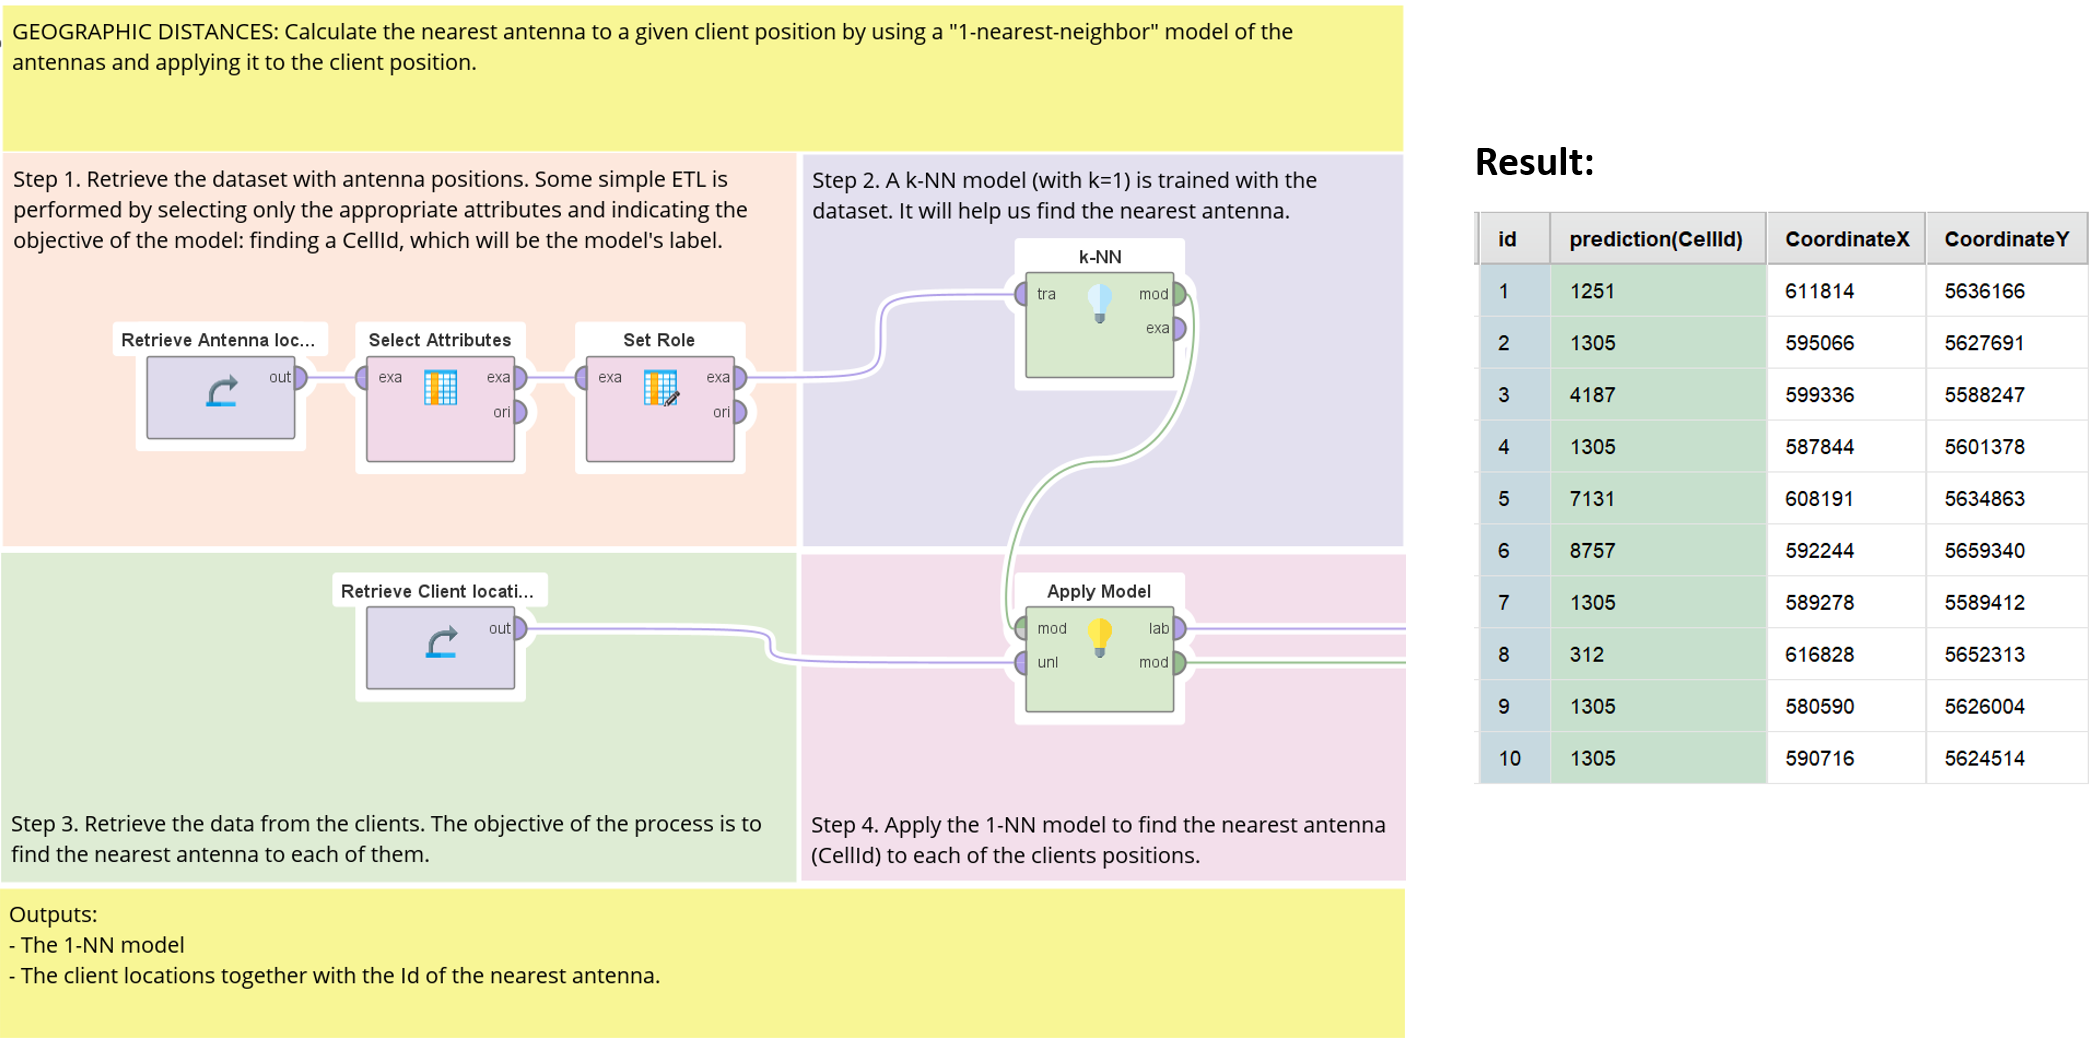
\includegraphics[height=0.6\paperheight]{images/Altair/Altair_proc_exmpl.png}
        \caption{How 3-NN method works}
    \end{figure}
\end{frame}
